\newcommand{\timestack}[0]{\textit{timestack} }
% \newcommand{\frame}[0]{\textit{frame} }
\newcommand{\threshold}[0]{\textit{threshold} }

\paragraph{}Os métodos apresentados no Capítulo 2 agora serão utilizadas em conjunto para estimar a altura de ondas do mar. Este algoritmo é composto de três etapas: o pré-processamento, o processamento principal, e a análise da imagem resultante. Estas etapas serão detalhadas nas seções a seguir.

\section{Pré-Processamento}

\begin{figure}[h]
  \subfloat[\textit{Pipeline} do pré-processamento.]{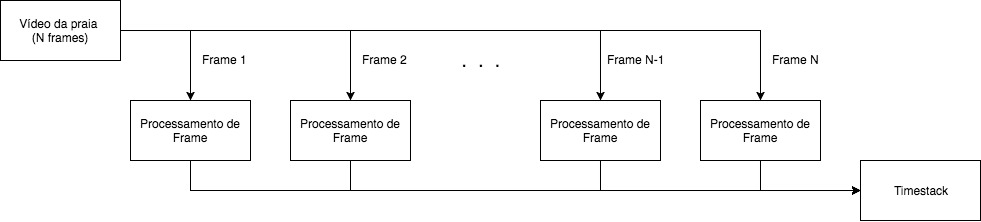
\includegraphics[width=\textwidth,keepaspectratio]{pre_processamento_pipeline.png}}
  \qquad
  \subfloat[Processamento de cada \textit{frame}.]{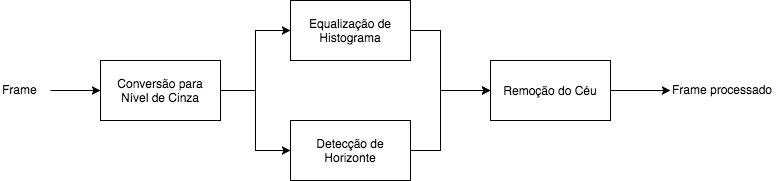
\includegraphics[width=\textwidth,keepaspectratio]{pre_processamento_frame.png}}
  \caption[\small{Diagrama de Bloco da etapa de pré-processamento.}]{\small{Diagrama de Bloco da etapa de pré-processamento.}}
  \label{FigDiagramaPreProc}
\end{figure}

\paragraph{}A etapa de pré-processamento tem como objetivo transformar os dados de entrada (o vídeo capturado de uma praia) em uma imagem \timestack  pronta para ser processada e analisada pelos passos subsequentes. O pré-processamento atua sobre cada \textit{frame} do vídeo, realizando as seguintes operações: conversão para nível de cinza, equalização de histograma, detecção da linha de horizonte, remoção do céu. Após operar cada \textit{frame} do vídeo é gerado um \timestack das imagens processadas. A figura \ref{FigDiagramaPreProc} ilustra os passos realizados.

\paragraph{}O passo mais importante nessa etapa é a criação do \timestack, que é uma representação espaço-temporal de um vídeo. O \timestack é a imagem que será processada pelo processamento principal e analisada para extração dos dados das ondas do mar. Os demais passos servirão para garantir a confiabilidade do \timestack e o prepararão para a etapa de processamento principal.

\paragraph{}O pré-processamento inicia a partir do vídeo capturado de uma praia. Cada \textit{frame} do vídeo é processado, primeiro convertendo o \textit{frame} para uma imagem em níveis de cinza, pois todos os processamentos posteriores só operam sobre o nível de intensidade de cada \textit{pixel}. A seguir, equaliza-se o histograma do \textit{frame}, a fim de normalizar a iluminação da imagem. Esta operação é necessária para possibilitar que filmagens realizadas em qualquer hora do dia podem ser tratadas da mesma forma. Os passos seguintes são a detecção da linha do horizonte e a remoção do céu. Para detectar o horizonte, analisa-se o \frame original em nível de cinza. Uma vez detectada a linha do horizonte, o céu é removido simplesmente alterando todos \textit{pixels} acima da linha para intensidade zero. O último passo é gerar o \timestack a partir dos \textit{frames} do vídeo. O \timestack é gerado selecionando a coluna central de cada \textit{frame}, acumulando-as sequencialmente em uma única imagem. Todos esses passos serão descritos detalhadamente a seguir.

\section{\textit{Timestack}}

\paragraph{}Um \timestack é uma representação bidimensional de um vídeo, isto é, trata-se de uma forma de transformar tal vídeo em uma só imagem. O \timestack é útil para analisar tais vídeos pois é possível olhar para uma sequência completa de quadros observando uma única imagem. Dessa forma, pode-se aplicar métodos de processamento de uma única imagem \timestack, em vez de todo o vídeo.

\paragraph{}Para construir um \timestack, é necessário fixar uma das dimensões espaciais de cada imagem do vídeo, obtendo assim um conjunto de funções unidimensionais. O \timestack deste vídeo é definido então como uma função bidimensional \(s_{Y}(x,t)\) ou \(s_{X}(t,y)\), onde \(x\) e \(y\) são coordenadas espaciais; \(t\) é uma coordenada temporal; as amplitudes \(s_{X}\) e \(s_{Y}\) são a intensidade ou nível de cinza do vídeo \(g(x,y,t)\) quando são fixados os valores \(x = X\) e \(y = Y\), respectivamente. Dessa forma, a relação entre um \timestack e um vídeo é dada por: \(s_{Y}(x,t)=g(x,Y,t)\) e \(s_{X}(t,y) = g(X,y,t)\).

\begin{figure}[h]
\begin{center}
  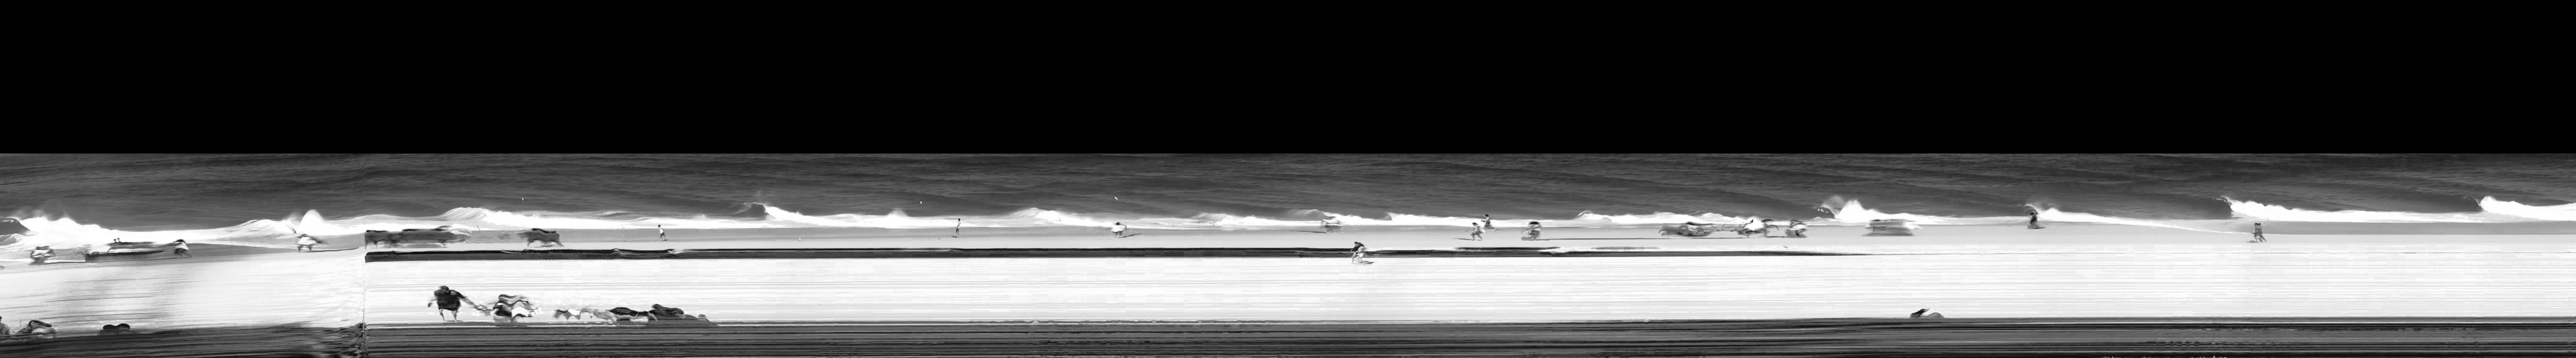
\includegraphics[width=\textwidth,keepaspectratio]{timestack.jpg}
  \caption[\small{\textit{Timestack} resultante do pré-processamento a partir do vídeo de uma praia.}]{\small{\textit{Timestack} resultante do pré-processamento a partir do vídeo de uma praia.}}
  \label{FigTimestack}
\end{center}
\end{figure}

\paragraph{}Note que, na prática, a coordenada temporal \(t\) cumpre o papel de uma coordenada espacial quando o \timestack é exibido como uma imagem, mas sua interpretação continua sendo temporal. Como é possível notar na figura \ref{FigTimestack}, cada onda aparenta crescer a medida que se desloca da esquerda para a direita e de cima para baixo. Isso ocorre pois o deslocamento horizontal representa a evolução temporal da onda, representa eventos que estão ocorrendo sequencialmente, primeiro a onda cresce até que chega no seu ponto máximo e quebra. O deslocamento vertical representa o avanço da onda até quebrar na areia da praia.

\paragraph{}É importante lembrar que a perda de uma dimensão resulta em perda de informação no vídeo, entretanto, nos casos em que o vídeo se mantém constante na dimensão espacial fixada não há perda de informação. Expandindo esse conceito, nos casos em que o vídeo varie muito pouco em uma de suas dimensões espaciais, não há necessariamente uma perda de conteúdo significativa.

\paragraph{}A análise de ondas marítimas apresenta condição similar a descrita anteriormente. Com a posição da câmera escolhida com cuidado, isto é, a zona de arrebentação deve centralizada na imagem, tanto horizontalmente quando verticalmente. A câmera deve estar perpendicular em relação a zona de arrebentação, e montada em um ponto acima do nível da praia, de forma que banhistas na areia não atrapalhem a visão da zona de arrebentação. Assim, uma onda quebrando ocupará maior parte horizontal da imagem. Além disso, não é importante para a análise desejada entender o tamanho horizontal da onda, apenas o seu tamanho vertical. Precisa-se apenas determinar o seu ponto mais baixo e seu ponto mais alto. Sendo assim, o \timestack mostra-se um método adequado de análise de vídeos para esse projeto.

\section{Aparato Instrumental}

% Está esquecendo do seu trabalho de projeto integrado. Trazer ele para cá fazendo referência aos seus colegas co-autores.

\paragraph{}Como mencionado anteriormente este projeto foi concebido como parte do sistema de monitoramento de praias \textit{GoSurf}, sendo o monitoramento por imagens apenas uma parte do sistema. Esse sistema foi criado para a disciplina Projeto Integrado no ano letivo 2015.1, em conjunto com outro aluno, Filipe Barretto. Para este fim foi desenvolvido um aparato instrumental que adquire dos dados e os analisa previamente por meio de uma central de processamento de dados, e por fim os envia para um servidor na nuvem. O servidor finaliza o processamento dos dados e disponibiliza para os resultados para os usuários por um aplicativo \textit{Android}.

\paragraph{}

%Neste (Não está claro para mim se é o GoSurf ou o PdG)%

projeto as imagens foram adquiridas de duas formas: através de câmeras de \textit{smartphones} comuns e através da câmera montada no \textit{hardware} apresentado anteriormente. Embora para este projeto a câmera de \textit{smartphones} atenda o requisito, o aparato instrumental é fundamental para o projeto \textit{GoSurf} completo porque agrega sensores extra além da câmera. Outra vantagem do aparato sensorial é a capacidade de realizar o pré-processamento localmente, o que reduz drasticamente o volume de dados que devem ser enviado ao servidor. Por exemplo, um vídeo de 125MB é reduzido para uma imagem de 657KB.

%Observe que a intenção desta seção de aparato instrumental é mostrar o hardware utilizado. Aqui você apenas mencionou que existe um hardware. Descreva aqui o hardware do seu experimento.

\section{Estabilização de Vídeo}

\paragraph{}A estabilização do vídeo é fundamental para a criação de um \timestack fiel ao cenário real. Esta necessidade surge uma vez que o \timestack é criado selecionando a coluna central de cada \textit{frame} do vídeo, tornando importante que esta coluna corresponda ao mesmo conjunto de pixels de quadro a quadro. Caso a câmera se desloque horizontalmente no decorrer do vídeo, o conjunto de pixels não será o mesmo, e com isso o \timestack formado não será uma representação fiel em duas dimensões do vídeo capturado. A estabilidade na direção vertical é importante para que a estimativa de altura das ondas seja fiel a altura real. Um deslocamento vertical da câmera resulta em um deslocamento das colunas do \timestack, que por sua vez podem embutir erros na identificação dos pontos de máximo e mínimo de cada onda.

\paragraph{}Primeiro experimentou-se realizar a estabilização do vídeo utilizando técnicas de processamento de imagens. Foi testado um procedimento simples descrito por Nghia Ho \cite{Ho2014}. Embora este procedimento apresente bons resultados para vídeos gravados manualmente, foi observado que quando aplicado o procedimento em vídeos gravados já com alta estabilidade o procedimento introduzia erros no \timestack resultante. Então, concluiu-se que basta utilizar um ponto de montagem para a câmera, como um tripé, para atingir a estabilidade necessária para a extração fiel dos dados desejados.

%Colocar imagens descritivas deste último parágrafo e referenciá-las. O texto explica o problema mas não permite ao leitor construir uma imagem mental do problema.

\section{Conversão para Nível de Cinza}

\paragraph{}Após gerar o \timestack, o mesmo é convertido para nível de cinza. Os passos e etapas subsequentes do algoritmo ora proposto não necessitam trabalhar com cores, apenas a intensidade de cada \textit{pixel} é necessária para estimar a altura das ondas. O processamento das imagens se torna mais eficiente, pois a representação de uma imagem em nível de cinza possui um terço do tamanho de representação de imagem em cores. Com isso, o algoritmo utilizara menos memória para executar e seu tempo de execução é reduzido.

\paragraph{}A conversão para nível de cinza é realizada de acordo com a seguinte fórmula \cite{Griffith14}:

\[
  I(t, v) = 0.35R(t, v) + 0.5G(t, v) + 0.15B(t, v)
\]

\noindent{}onde \(I(t,v)\) é a intensidade do pixel na posição \((t,v)\) na imagem convertida, e \(R(t,v)\), \(G(t,v)\) e \(B(t,v)\) são, respectivamente, os valores das componentes vermelhas, verdes e azuis do pixel \((t,v)\) da imagem original.

\section{Equalização de Histograma}

\paragraph{}A equalização de histograma tem como funcionalidade normalizar o nível intensidade da imagem. Desta forma, reduz-se tanto o efeito do clima (como a variação da iluminação em dias nublados e dias de céu aberto) quanto o efeito do horário do dia (como a variação da iluminação entre o começo da manhã e o meio do dia). Além disso, nuvens e objetos externos podem alterar a iluminação durante a aquisição do vídeo em si. Portanto, deve-se equalizar o histograma de cada \textit{frame} do vídeo antes de gerar o \textit{timestack}.

%Descrever como é feita a equalização, tal como você fez na seção de níveis de cinza.

\section{Detecção da Linha de Horizonte}

\paragraph{}Uma etapa importante é a detecção da linha de horizonte a fim de viabilizar a detecção e remoção do céu na imagem. Esta operação é utilizada para facilitar o passo de \textit{thresholding} na etapa de processamento de imagem. Em alguns cenários, é difícil distinguir a região de céu da região de arrebentação utilizando apenas o nível de intensidade dos \textit{pixels} de cada região, pois a faixa de valores de intensidade de cada região se sobrepõem. A figura \ref{FigTimestackFail}a exibe um \timestack com o céu incluído após aplicado um \textit{threshold} com valor de limite 150. Pode-se observar que parte do céu não foi removido pelo \textit{threshold} (faixa branca na parte superior da imagem). Já a figura \ref{FigTimestackFail}b exibe um \timestack com o céu incluído após aplicado um \textit{threshold} com valor de limite 210. Com este valor o céu foi removido completamente, mas a delimitação da região de espuma não foi bem definida, dificultando ou até impossibilitando sua identificação (observe a faixa preta estreita presente na faixa branca da imagem). Por este motivo, a segmentação é baseada não só no nível de intensidade dos \textit{pixels} mas como na sua localização na imagem. A detecção da linha de horizonte se mostra fundamental para obter localização desta região.

\begin{figure}[h]
  \centering
  \subfloat[\small{\textit{Timestack} sem remoção do céu (valor de \textit{threshold} 150)}]{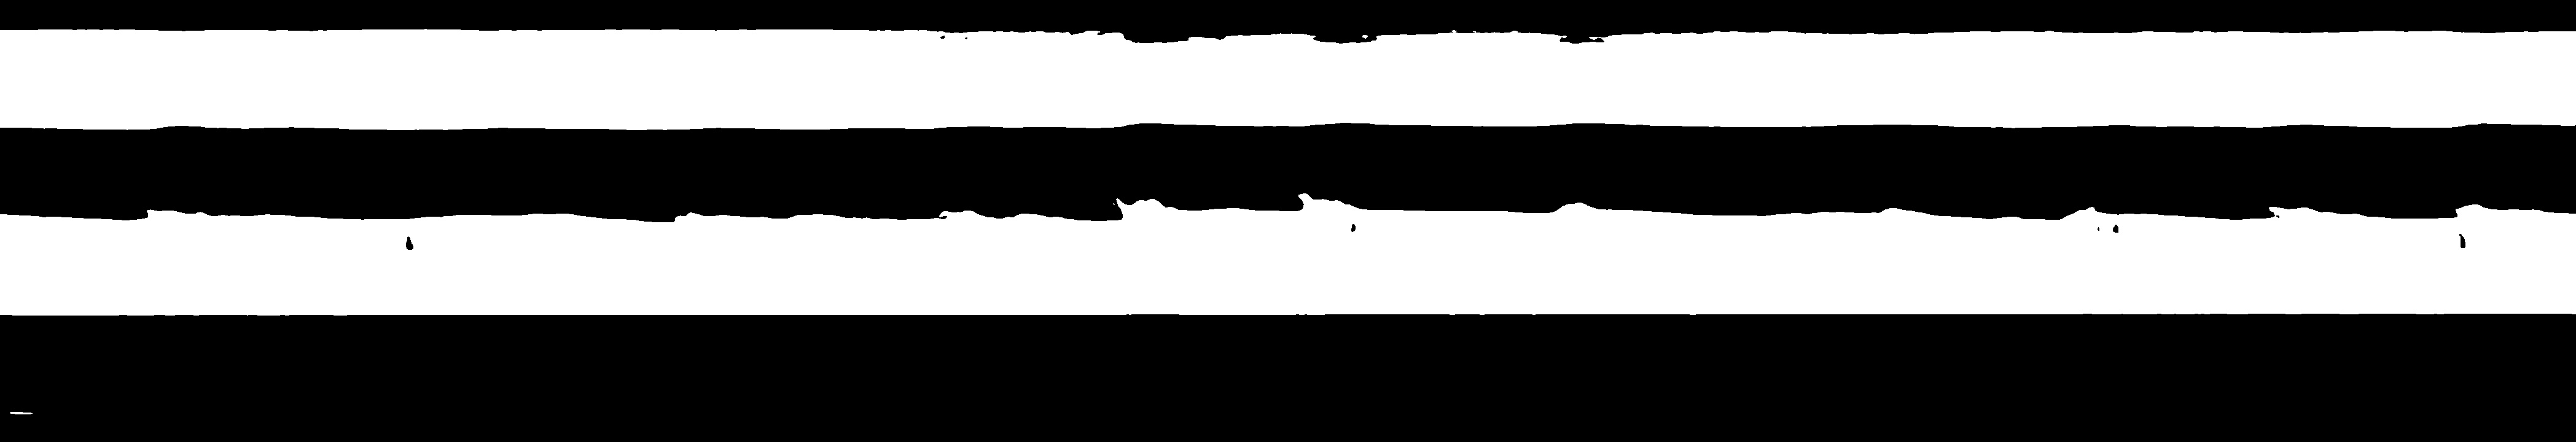
\includegraphics[width=\textwidth,keepaspectratio]{process_threshold_150.jpg}}
  \qquad
  \subfloat[\small{\textit{Timestack} sem remoção do céu (valor de \textit{threshold} 210)}]{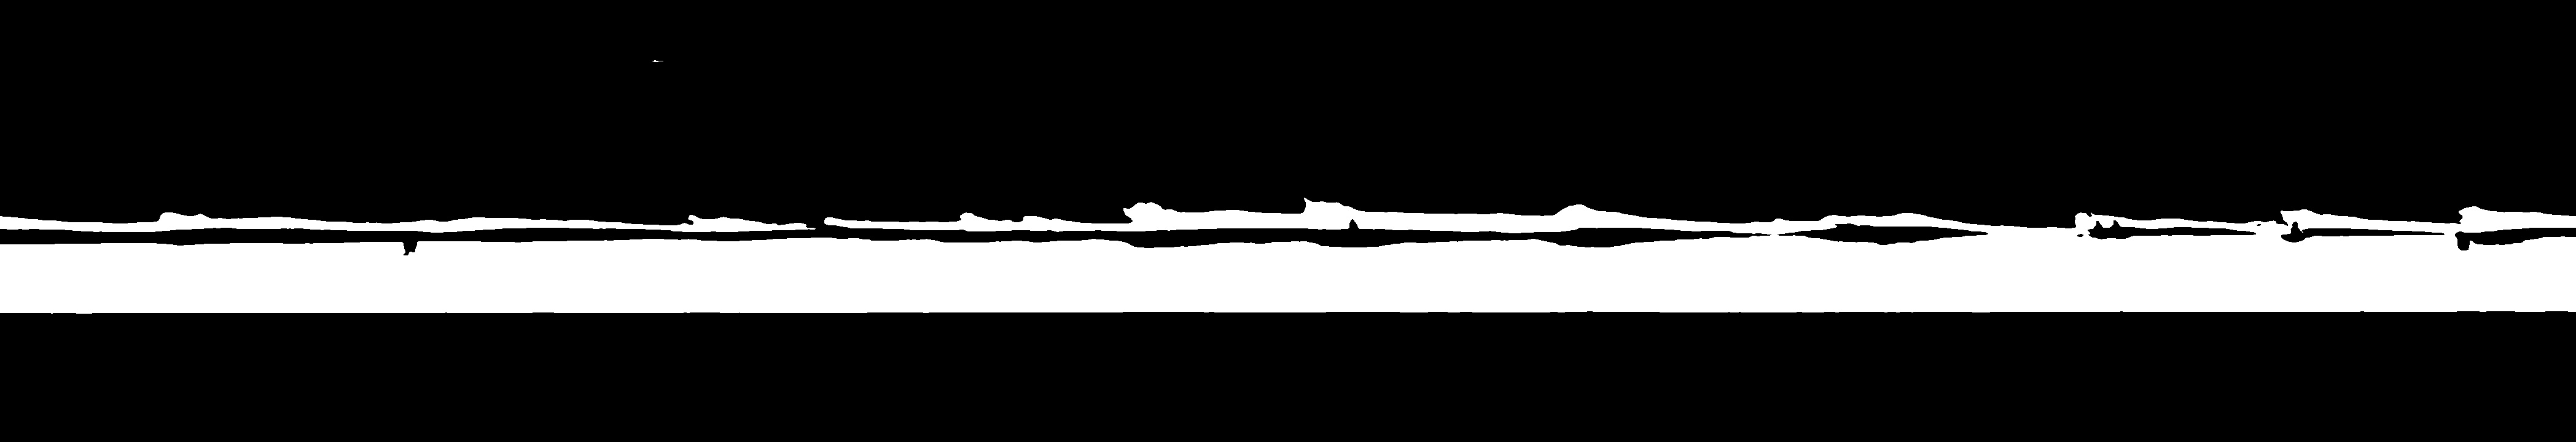
\includegraphics[width=\textwidth,keepaspectratio]{process_threshold_210.jpg}}
  \caption[\small{Comparação do resultado do passo de \textit{thresholding} sem a remoção do céu.}]{\small{Comparação do resultado do passo de \textit{thresholding} sem a remoção do céu.}}
  \label{FigTimestackFail}
\end{figure}

\paragraph{}A detecção do céu é realizada utilizando um detector de bordas de Canny para identificar a borda entre o céu e o mar em um \textit{frame} do vídeo (Figura \ref{FigFrameCanny}). Então, procura-se a primeira borda detectada pelo método de Canny, através do algoritmo descrito em \ref{AlgLineTracking}. A borda detectada corresponde a linha do horizonte. Todos os \textit{pixels} acima dessa linha são considerados como \textit{pixels} da região do céu, e serão removidos no passo seguinte.

%Colocar a imagem original junto com a figura abaixo.

\begin{figure}[h]
  \centering
  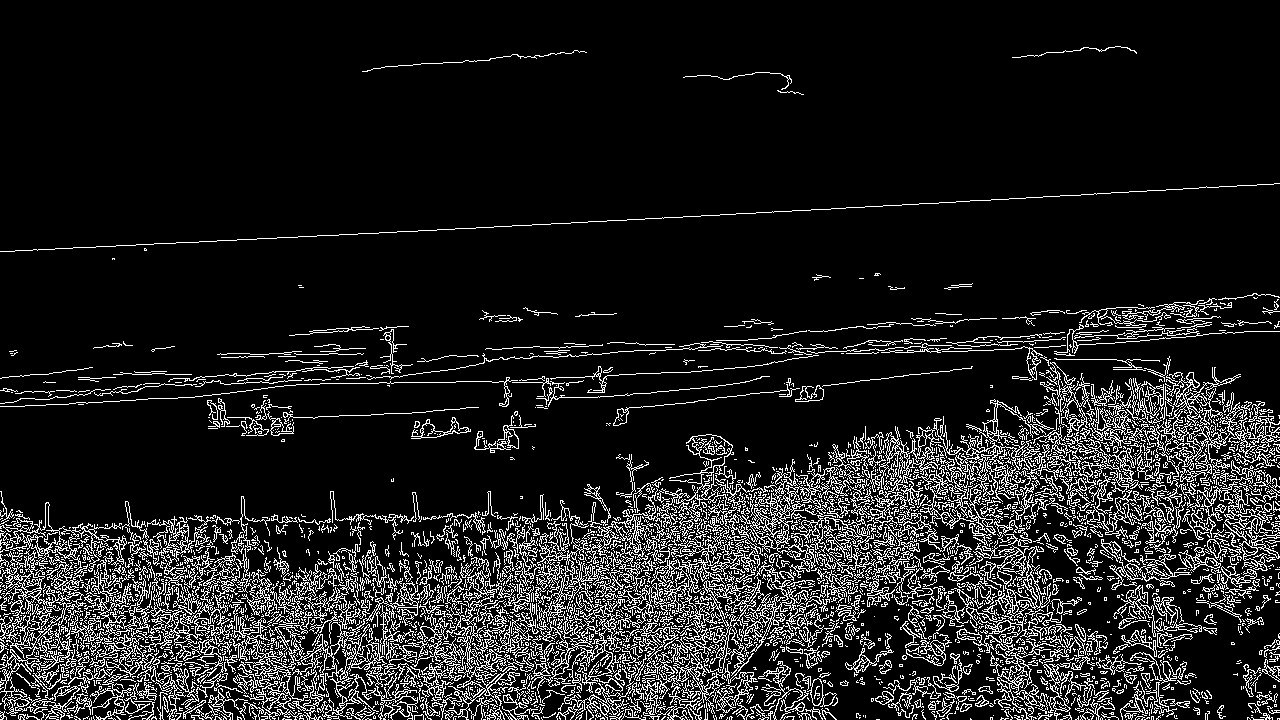
\includegraphics[width=0.8\textwidth,keepaspectratio]{simpletimestack_canny.jpg}
  \caption[\small{\textit{Frame} do vídeo com bordas detectadas pelo método de Canny. A primeira borda identificada é a linha do horizonte.}]{\small{\textit{Frame} do vídeo com bordas detectadas pelo método de Canny. A primeira borda identificada é a linha do horizonte.}}
  \label{FigFrameCanny}
\end{figure}

\section{Remoção do Céu}

\paragraph{}O último passo da etapa de pré-processamento é a remoção do céu. Este passo utiliza duas entradas, a linha do horizonte detectada pelo passo anterior, e o \textit{frame} equalizado. A partir da linha do horizonte, considera-se todos os \textit{pixels} do \textit{frame} equalizado acima dessa linha como preto. A figura \ref{FigFrameSkyRemoved} exibe um \textit{frame} equalizado do vídeo original com o céu removido.

\begin{figure}[h]
  \centering
  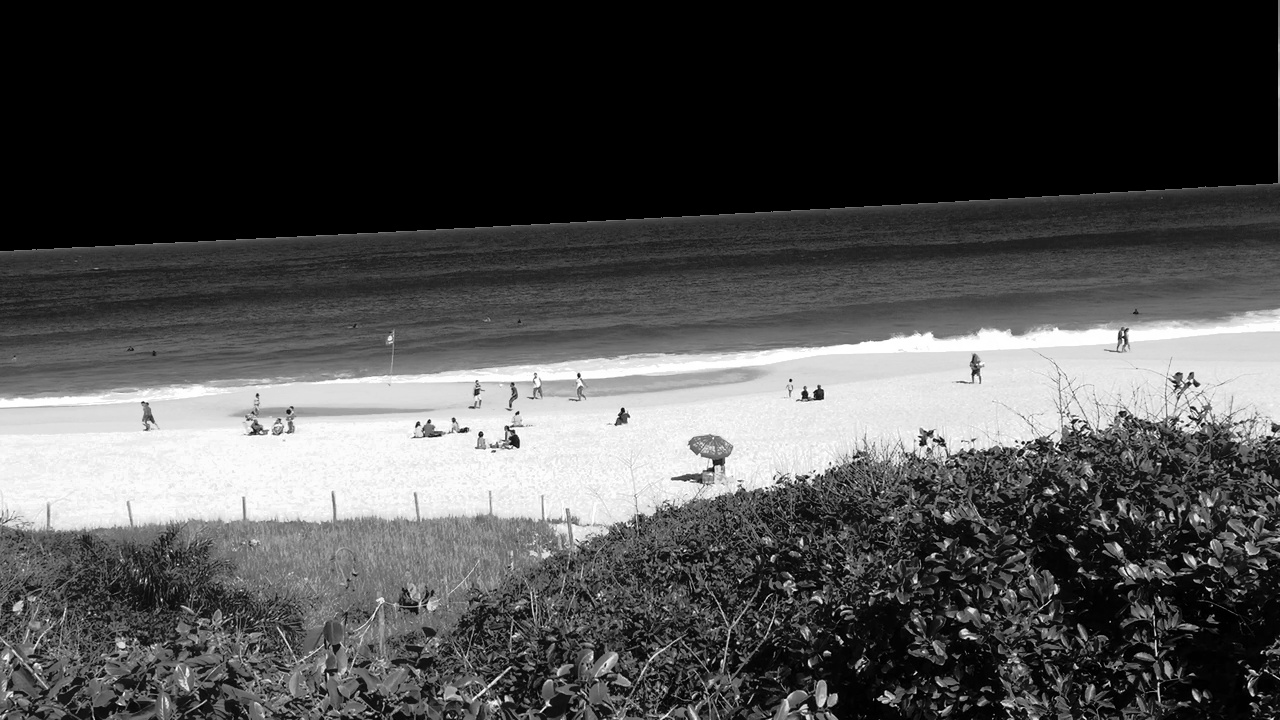
\includegraphics[width=0.8\textwidth,keepaspectratio]{simpletimestack_sky_removed.jpg}
  \caption[\small{\textit{Frame} equalizado com o céu removido}]{\small{\textit{Frame} equalizado com o céu removido}}
  \label{FigFrameSkyRemoved}
\end{figure}

\paragraph{}Como dito anteriormente, sem a remoção do céu, é difícil definir um valor único de \textit{threshold} que será utilizado na etapa de processamento principal. Uma tarefa essencial é ser capaz de separar o céu, o mar e a faixa de espuma da arrebentação. Com o céu removido, ao operação de \textit{threshold} produzirá resultados mais adequados para dar suporte às etapas de medição.

\section{Processamento Principal}

\begin{figure}[h]
\begin{center}
  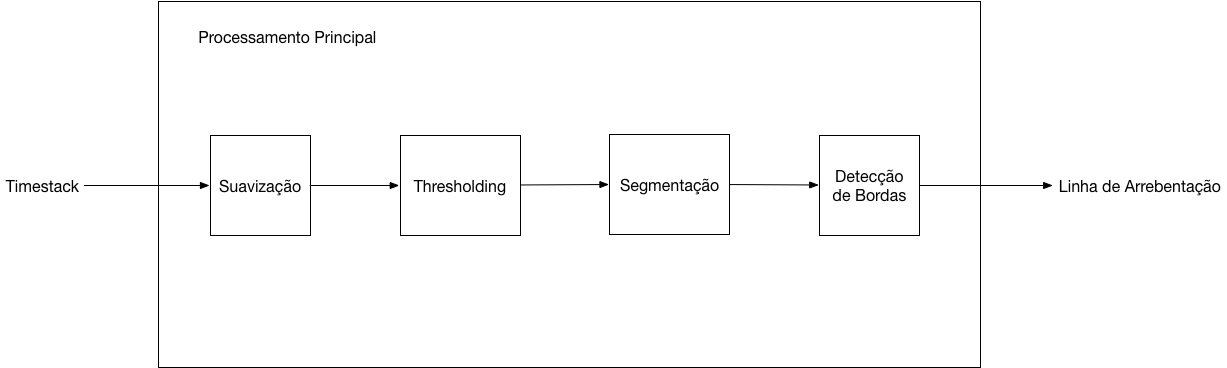
\includegraphics[width=\textwidth,height=\textheight,keepaspectratio]{diagrama_processamento.png}
  \caption[\small{Diagrama de Bloco da etapa de processamento principal.}]{\label{FigDiagramaProc} \small{Diagrama de Bloco da etapa de processamento principal.}}
\end{center}
\end{figure}

\paragraph{}A etapa de processamento principal tem como objetivo extrair a linha de arrebentação (figura \ref{FigLinhaArrebentacao}) de um \timestack gerado pelo pré-processamento. A linha de arrebentação é definida como a linha que delimita a região de espuma do restante do mar. Uma característica marcante dessas duas regiões é que a região de espuma apresenta a maioria dos \textit{pixels} com intensidade alta, enquanto o restante do mar apresenta a maioria dos \textit{pixels} com intensidade baixa. Esta característica será explorada para separar a região de espuma do restante da imagem. Em seguida, a borda superior desta região, que corresponde a linha de arrebentação, será analisada para identificar as ondas do mar presentes na imagem e medir a sua altura e periodicidade.

%Colocar junto com a imagem a seguir, a imagem equalizada e sem céu que foi utilizada.

\begin{figure}[h]
\begin{center}
  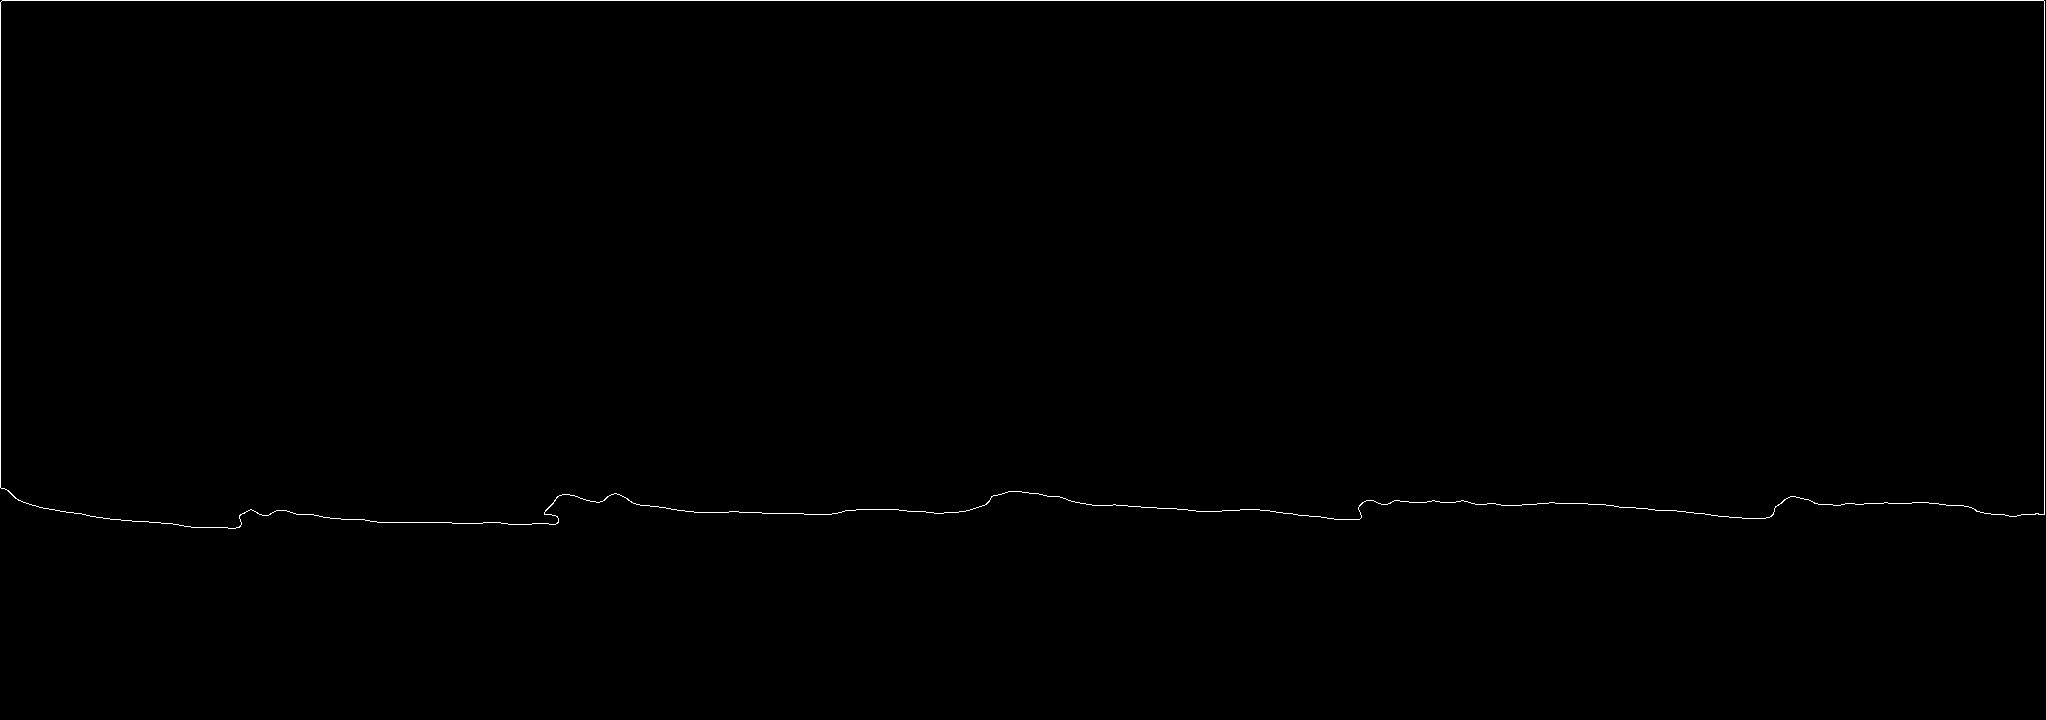
\includegraphics[width=\textwidth,height=\textheight,keepaspectratio]{mainprocessing_breakzone_line.jpg}
  \caption[\small{Linha de arrebentação detectada pelo processamento principal.}]{\label{FigLinhaArrebentacao} \small{Linha de arrebentação detectada pelo processamento principal.}}
\end{center}
\end{figure}

\paragraph{}As etapas de suavização, \textit{thresholding}, segmentação e detecção de bordas, que compõe o Processamento Principal, serão descritas nas seções a seguir.

\section{Suavização}

\paragraph{}A primeira etapa de suavização é realizada utilizando um filtro passa-baixas gaussiano, implementado no domínio do espaço com máscara de tamanho 15, valor escolhido empiricamente após experimentar com imagens de diversos dias diferentes. Este efeito de suavização é importante para reduzir o nível de ruído na imagem, facilitando a identificação das bordas relevantes nos passos subsequentes. Outro efeito desejado é homogeneizar o nível de intensidade das regiões da imagem, de forma que o passo de \textit{thresholding} consiga segmentar a região de arrebentação do \timestack consistentemente. A figura \ref{FigGaussianBlurComparison} ilustra a diferença na segmentação da região de espuma com e sem o passo de suavização. A região de espuma detectada está marcada em vermelho. Nota-se que na figura \ref{FigGaussianBlurComparison}b a região de espuma detectada é influenciada por pequenas faixas de alta intensidade espalhadas na região do mar, enquanto a figura \ref{FigGaussianBlurComparison}a consegue filtrar essa influência e detectar uma região de espuma mais uniforme.

\begin{figure}[h]
  \centering
  \subfloat[Região de espuma detectada em um \textit{timestack} suavizado.]{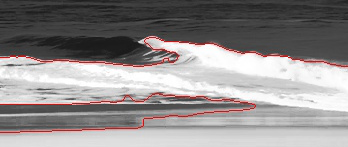
\includegraphics[width=0.8\textwidth,keepaspectratio]{waveband_blur.png}}
  \qquad
  \subfloat[Região de espuma detectada em um \textit{timestack} não-suavizado.]{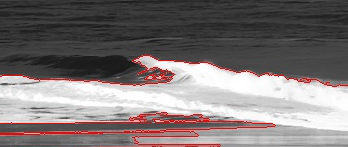
\includegraphics[width=0.8\textwidth,keepaspectratio]{waveband_no_blur.png}}
  \caption[\small{Comparação da região de espuma detectada com e sem suavização.}]{\small{Comparação da região de espuma detectada com e sem suavização.}}
  \label{FigGaussianBlurComparison} 
\end{figure}

%TODO: Adicionar imagem da primeira suavização

\section{\textit{Thresholding}}

\paragraph{}\textit{Thresholding} é o primeiro passo para realizar a segmentação. Neste passo separa-se a região de espuma do restante do mar, alterando todos os \textit{pixels} com intensidade abaixo de 150 para 0, e todos os \textit{pixels} acima deste valor para o valor de intensidade máximo. O valor limite foi escolhido empiricamente após a análise de diversas imagens, contemplando dias variados. A figura \ref{FigThreshold} compara a região de espuma detectada após o passo de \textit{threshold} com valores diferentes. Pode-se notar na figura \ref{FigThreshold}a uma borda mais estreita sobre a região de espuma observada, enquanto a figura \ref{FigThreshold}b exibe uma região detectada não condizente com o resultado esperado. Inicialmente foi considerado um método de decisão do valor de \threshold dinâmico, mas como discutido previamente, os passos de equalização e remoção do céu realizados durante o pré-processamento permitem utilizar um valor de \threshold estático, independente da condição de iluminação no momento da aquisição do vídeo. 

\paragraph{}Entretanto, dias muito nublados podem causar problemas para o \textit{thresholding}, como pode ser visto na figura \ref{FigThresholdFail}. Nesta figura os valores de intensidade da região de espuma e da região do mar no entorno das ondas se sobrepõe. Neste caso, o \threshold com valor estático não é capaz de separar as duas regiões, impossibilitando a identificação das ondas do mar nos passos subsequentes.

\paragraph{}É importante notar que o \textit{thresholding} apenas isola as regiões cujo nível de intensidade está acima de um certo valor. Mais de uma região pode ser isolada durante esse processo, por exemplo, partes da região do mar pode estar mais clara que o esperado, e por isso serão preservadas pelo \threshold. O passo de segmentação é responsável por filtrar as regiões isoladas pelo \textit{thresholding}.

%Atualizar essa figura

\begin{figure}[h]
  \centering
  \subfloat[\small{Região de espuma detectada usando \textit{threshold} no valor 150.}]{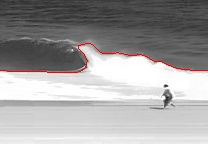
\includegraphics[width=.4\textwidth,keepaspectratio]{waveband_threshold_150.png}}
  \qquad
  \subfloat[\small{Região de espuma detectada usando \textit{threshold} no valor 120.}]{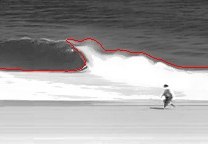
\includegraphics[width=.4\textwidth,keepaspectratio]{waveband_threshold_120.png}}
  \caption[\small{Trecho de um \textit{timestack} após aplicação de um \textit{threshold} com valores diferentes.}]{\small{Trecho de um \textit{timestack} após aplicação de um \textit{threshold} com valores diferentes.}
  \label{FigThreshold}
}
\end{figure}

\section{Segmentação e Detecção de Bordas}

\paragraph{}O último passo do processamento principal é a segmentação. Este passo tem como objetivo identificar a região de espuma dentre as regiões isoladas pelo \textit{thresholding}, e identificar a sua borda externa para ser analisada pela próxima etapa. Primeiro, deve-se identificar todas as regiões isoladas pelo \textit{thresholding}. Como a imagem está binarizada, isto é, todos \textit{pixels} possuem a intensidade mínima ou máxima, as regiões isoladas serão os conjuntos de \textit{pixels} contínuos com intensidade máxima. 

%Mostrar um pseudo código, ou mesmo o código, de como isso foi implementado.

\paragraph{}Em seguida, calcula-se a área de cada região, a fim de encontrar a região com a maior área. 

%Mostrar um pseudo código, ou mesmo o código, de como isso foi implementado.

\paragraph{}Em condições normais a região de maior área será a região de espuma da imagem, então pode-se descartar todas as outras regiões. Por fim basta identificar as bordas da região restante utilizando um método de detecção de bordas. Para facilitar a implementação foi utilizado o método de Suzuki \cite{Suzuki85} para detecção da borda, pois esse método já está implementado na biblioteca \textit{OpenCV}. Outro método considerado para esta tarefa é o detector de bordas de Canny, já utilizado no passo de detecção da linha do horizonte, mas que neste caso não obteve resultados tão bons quanto o método de Suzuki.

%Mostrar imagem da borda detectada com Suzuki e com Canny.

\section{Análise e Identificação das Ondas Marítimas}

\paragraph{}A última etapa do algoritmo de estimação da altura de ondas do mar é analisar a linha de arrebentação extraída do \timestack e identificar as ondas do mar presentes nesta imagem. Feito isso, é possível encontrar o ponto mínimo e máximo locais da linha de arrebentação, que correspondem ao ponto mínimo e máximo da onda em questão. Estas etapas são descritas nas seções a seguir.

\begin{figure}[h]
\begin{center}
  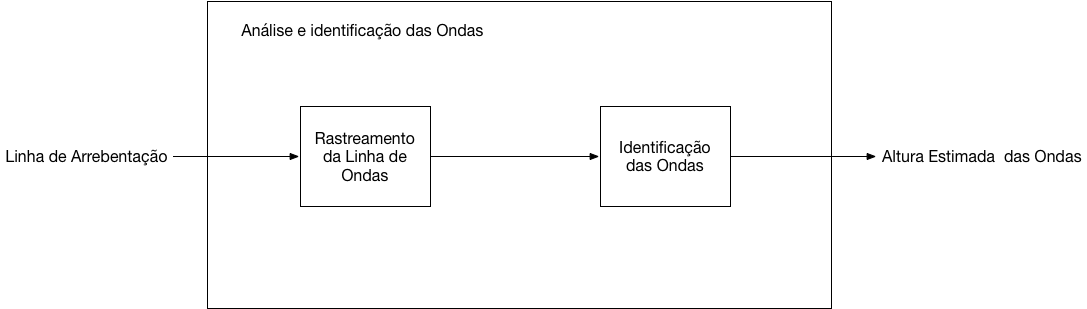
\includegraphics[width=\textwidth,height=\textheight,keepaspectratio]{diagrama_analise.png}
  \caption[\small{Diagrama de Bloco da etapa de análise. Fonte: Autor}]{\label{FigDiagramaAnalise} \small{Diagrama de Bloco da etapa de análise.}}
\end{center}
\end{figure}

\section{Rastreamento da Linha de Ondas}

\paragraph{}O primeiro passo desta etapa consiste em rastrear a linha de arrebentação encontrada, isto é, construir uma sequência \(s[n]\) que indica a sequência ordenada dos pontos \((x,y)\) que compõe a linha de arrebentação. Esta sequência ordenada permite caminhar por cima da linha de arrebentação e assim determinar os pontos de máximo e mínimo locais da linha.

\paragraph{}Para rastrear a linha de arrebentação foi utilizado um algoritmo que, dado um ponto de origem \(s[0] = (x_{i},y_{i})\), encontra o próximo ponto da linha, o adiciona a sequência e busca o próximo ponto, até que não encontre mais nenhum ponto disponível para adicionar na sequência \(s[n]\). O primeiro ponto é encontrado simplesmente percorrendo coluna a coluna da imagem, a partir da coluna mais à esquerda até a coluna mais à direita até que se encontre um ponto de intensidade maior que zero. Então cria-se uma nova sequência com o ponto inicial igual ao ponto encontrado. O pseudo-código \ref{AlgFirstPoint} ilustra o algoritmo que encontra e popula o primeiro ponto ($s[0]$) de uma sequência $s[n]$. 

\paragraph{}A busca do próximo ponto ocorre na vizinhança imediata do último ponto da sequência, isto é, todos os oito pontos diretamente conectados ao ponto último ponto da sequência. Para cada ponto da sequência espera-se encontrar outros dois pontos em sua vizinhança, o ponto anterior e o ponto subsequente. Portanto, a análise da vizinhança deve desconsiderar o ponto anterior para não adicionar o mesmo ponto duas vezes na sequência. O ponto restante encontrado na vizinhança será o próximo ponto, então este ponto é adicionado ao final da sequência e o algoritmo se repete, até que mais nenhum ponto seja encontrado. Entretanto, é possível ocorrer descontinuidades na linha, isto é, um ponto na sequência possuir apenas um ou nenhum outro ponto em sua vizinhança imediata. Nesse caso, nenhum novo ponto será encontrado na vizinhança do último ponto da sequência, e o algoritmo será interrompido prematuramente. Para solucionar este problema se aumenta o raio da vizinhança e o algoritmo e repetido com o mesmo ponto central, buscando pontos mais distantes. Embora esta abordagem resolva os casos de descontinuidades pequenas, abre-se margem para que falsos positivos ocorram, isto é, pontos futuros sejam encontrados pulando o verdadeiro ponto subsequente. Para minimizar este problema, o raio de busca é limitado em um valor máximo igual a três.

\paragraph{}Outro problema que atrapalha o funcionamento do algoritmo de rastreamento são casos onde um ponto possui mais de dois pontos em sua vizinhança. Este problema acontece quando existe um "laço" na linha de arrebentação, e costuma ocorrer no momento que a onda quebra, e se torna mais comum a medida que o raio de busca aumenta. Nessa situação, considera-se o próximo ponto simplesmente o primeiro ponto novo encontrado na vizinhança, e os demais pontos encontrados não são considerados. Por último, existem regiões de espuma que o algoritmo não é capaz de rastrear a linha de arrebentação completamente, interrompendo a sequência prematuramente. Nesses casos, simplesmente inicia-se uma nova sequência a partir da coluna a direita do último ponto encontrado. Esse processo pode ser repetido inúmeras vezes até que se atinja a última coluna da imagem. O pseudo-código \ref{AlgLineTracking} ilustra o algoritmo de rastreamento que popula os pontos restantes de uma sequência $s[n]$.

\begin{algorithm}
  \caption{Algoritmo de Identificação do Primeiro Ponto da Linha}
  \label{AlgFirstPoint}
\begin{algorithmic}
\Procedure{EncontraPrimeiroPonto}{}
\For{cada coluna $c$ na borda da região de espuma}
        \For{cada elemento $e$ na coluna $c$}
                \If{intensidade do elemento $e > 0$}
                        \State $s[0] = \text{posição do elemento } e$
                        \State{fim}
                \EndIf
        \EndFor
\EndFor
\EndProcedure
\end{algorithmic}
\end{algorithm}

\begin{algorithm}
  \caption{Algoritmo de Rastreamento de Linha}
  \label{AlgLineTracking}
\begin{algorithmic}
\Procedure{RastreiaLinha}{$raioDeBusca$}
\State $PontoAtual \gets s[N]$ \Comment{último ponto de s[n]}
\For{ pontos p ao redor de $PontoAtual$ em um raio de $raioDeBusca$ } 
        \If { $p \neq 0$ e $p$ não está em $s[n]$ }
                \State $s[N+1] \gets p$
        \EndIf
\EndFor
\If{algum ponto foi adicionado a $s[n]$}
        \State{repetir o procedimento para o último ponto encontrado}
\Else
        \If{$raioDeBusca \leq 3$}
                \State{repetir o procedimento com $raioDeBusca+1$}
        \Else
                \State{fim}
        \EndIf
\EndIf
\EndProcedure
\end{algorithmic}
\end{algorithm}

\section{Identificação das Ondas}

\paragraph{}O último passo para estimar a altura das ondas em um \timestack é identificar as ondas na linha rastreada no passo anterior. Para isso, calcula-se a derivada da sequência discreta $s[n]$, da seguinte forma:

\[
  s'[n] = s[n] - s[n-1], \text{para n $>$ 0}
\] 

\noindent{}A sequência $s'[n]$ indica quais trechos da sequência original $s[n]$ são crescentes, decrescentes ou constantes. Então, ao caminhar sobre a sequência derivada $s'[n]$, é trivial determinar quais são as faces crescentes das ondas. Em um cenário ideal, o ponto inicial de uma face crescente corresponde ao ponto mínimo local de uma onda, e o último ponto crescente desta face corresponde ao ponto de máximo local, determinando assim a altura da onda. Entretanto, em uma imagem não ideal podem existir trechos que a derivada é $0$, ou até mesmo negativa, antes da sequência tornar a crescer. A figura \ref{FigAutomato} descreve um autômato que reconhece uma onda considerando as condições descritas anteriormente.

\begin{figure}[h]
\begin{center}
  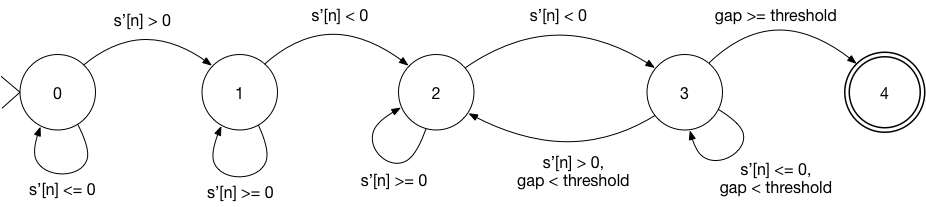
\includegraphics[width=\textwidth,height=\textheight,keepaspectratio]{automato_identificacao_onda.png}
  \caption[\small{Autômato Finito Determinístico que identifica uma onda em uma linha de arrebentação.}]{\label{FigAutomato} \small{Autômato Finito Determinístico que identifica uma onda em uma linha de arrebentação.}}
\end{center}
\end{figure}

\noindent{}O estado 0 do autômato procura pela primeira derivada $s'[n]$ positiva, marcando o ponto equivalente de $s[n]$ como o mínimo da onda e avançando para o estado 1. O estado 1 procura pela primeira derivada negativa de $s'[n]$, marcando o ponto equivalente de $s[n]$ como candidato ao ponto máximo da onda e andando para o estado 2. Então, os estados 2 e 3 buscam por "buracos" ou \textit{gaps} no trecho de derivada positiva, onde a derivada se torna negativa por um curto período e depois $s[n]$ torna a crescer. O estado 2 procura por novos pontos de máximo, trechos onde a derivada é positiva, e o estado 3 procura por trechos de derivada negativa. Quando o estado 3 encontrar uma derivada positiva, o autômato retorna para o estado 2. Enquanto o estado 3 encontrar derivadas não-positivas um contador de tamanho do \textit{gap} é incrementado. Quando o tamanho do \textit{gap} é superior a um certo limite, o autômato avança para o estado 4, identificando assim que um candidato a uma onda foi encontrado, delimitado pelos pontos de mínimo e máximo encontrados anteriormente. Este candidato apenas será considerado uma onda se sua altura estiver dentro de uma faixa de controle, isto é, são descartadas ondas muito pequenas ou muito grandes. A figura \ref{FigWave} mostra os pares de pontos máximo e mínimo identificados pelo autômato em uma linha de arrebentação aplicados no \timestack original. As linhas verdes unem os pares de pontos encontrados, e as linhas vermelhas evidencia a altura em \textit{pixels} da onda identificada. 

\begin{figure}[h]
\begin{center}
  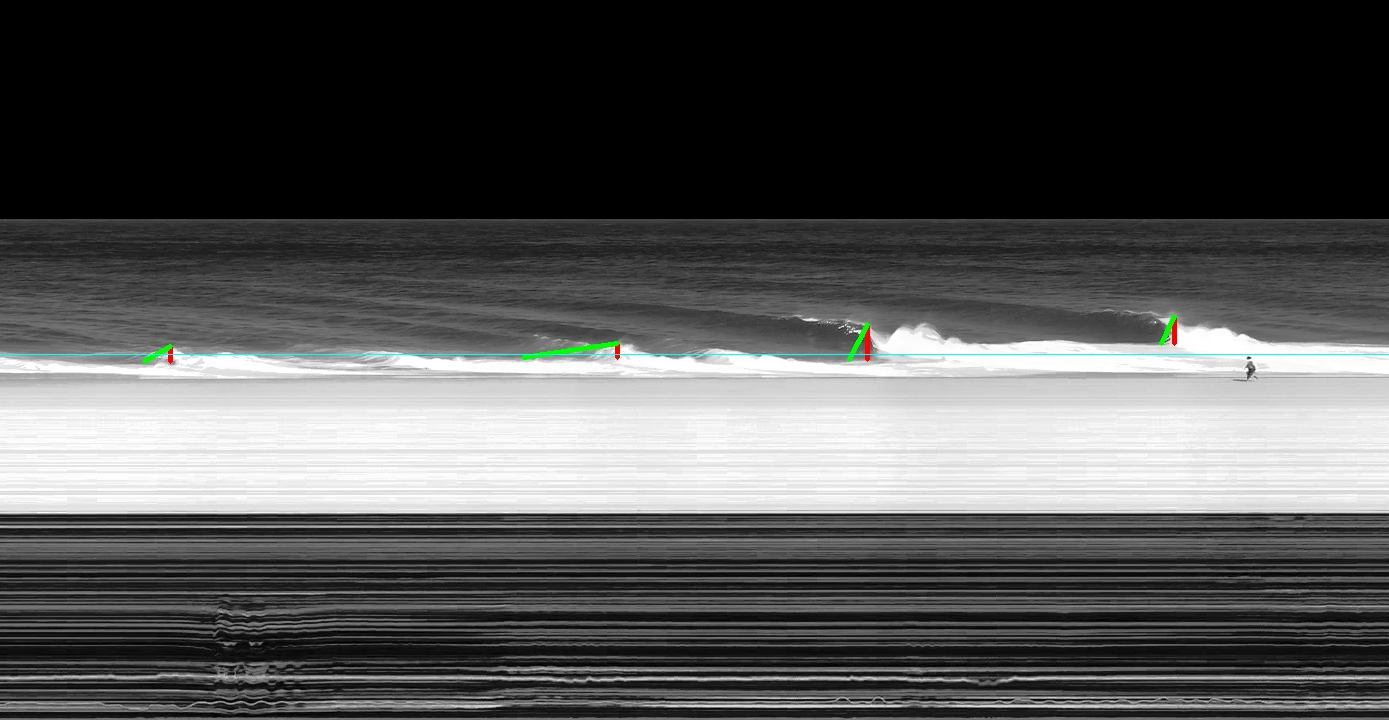
\includegraphics[width=\textwidth,height=\textheight,keepaspectratio]{process_waves_result.png}
  \caption[\small{Ondas identificadas pelo autômato.}]{\label{FigWave} \small{Ondas identificadas pelo autômato.}}
\end{center}
\end{figure}
